\documentclass{beamer}
\usepackage{ctex, hyperref}
\usepackage[T1]{fontenc}

% other packages
\usepackage{latexsym,amsmath,xcolor,multicol,booktabs,calligra}
\usepackage{graphicx,pstricks,listings,stackengine}
\usepackage[normalem]{ulem}

\author{userElaina}
\title{Chains: Crowdsource}
\institute{School of AI}
\date{2024.07.07}
\usepackage{JilinUniv}

\def\cmd#1{\texttt{\color{red}\footnotesize $\backslash$#1}}
\def\env#1{\texttt{\color{blue}\footnotesize #1}}
\definecolor{deepblue}{rgb}{0,0,0.5}
\definecolor{deepred}{rgb}{0.6,0,0}
\definecolor{deepgreen}{rgb}{0,0.5,0}
\definecolor{halfgray}{gray}{0.55}

\lstset{
    basicstyle=\ttfamily\small,
    keywordstyle=\bfseries\color{deepblue},
    emphstyle=\ttfamily\color{deepred},    % Custom highlighting style
    stringstyle=\color{deepgreen},
    numbers=left,
    numberstyle=\small\color{halfgray},
    rulesepcolor=\color{red!20!green!20!blue!20},
    frame=shadowbox,
}

\begin{document}

\kaishu
\begin{frame}
    \titlepage
    \begin{figure}[htpb]
        \begin{center}
            
\includegraphics[width=0.15\linewidth]{pic/Jilin_University_Logo.eps}
        \end{center}
    \end{figure}
\end{frame}

% \begin{frame}
% \tableofcontents[sectionstyle=show,subsectionstyle=show/shaded/hide,subsubsectionstyle=show/shaded/hide]
% \end{frame}

\section{Crowd}

% \begin{frame}{AutoCoT}
%     \begin{figure}[c]
%         \centering
%         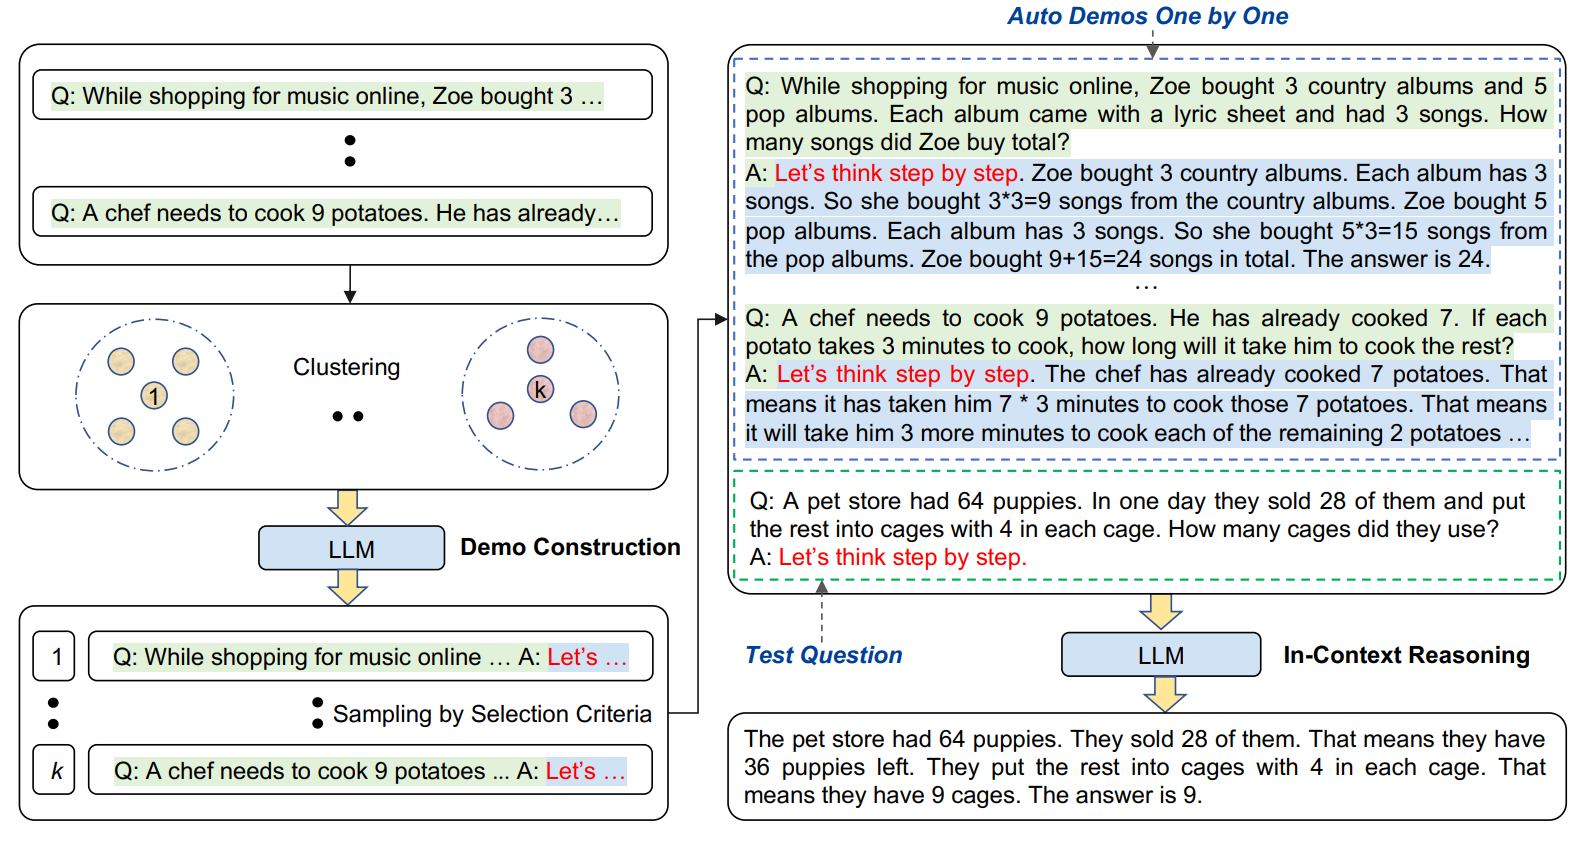
\includegraphics[height=.7\textheight]{pic/7.png}
%         \caption{Automatic Chain of Thought Prompting in Large Language Models}
%     \end{figure}
% \end{frame}

\begin{frame}{Crowd}
    \begin{itemize}
        \item 都是 $f(x) = w^Tx$. 需要其它的吗?
        \item 优化器: 用原来的? SGD / Adam? 不固定?
    \end{itemize}
\end{frame}

\begin{frame}{Experts}
    \begin{itemize}
        \item 固定 $\alpha_0=\beta_0=1$, 别的照常.
        \item 想法: 固定多个专家, 别的照常.
    \end{itemize}
\end{frame}

\end{document}

% Q model para
